\documentclass[a4paper,12pt]{article} % добавить leqno в [] для нумерации слева
\usepackage[a4paper,top=1.3cm,bottom=2cm,left=1.5cm,right=1.5cm,marginparwidth=0.75cm]{geometry}
%%% Работа с русским языком
\usepackage{cmap}					% поиск в PDF
\usepackage{mathtext} 				% русские буквы в фомулах
\usepackage[T2A]{fontenc}			% кодировка
\usepackage[utf8]{inputenc}			% кодировка исходного текста
\usepackage[english,russian]{babel}	% локализация и переносы

\usepackage{graphicx}

\usepackage{wrapfig}
\usepackage{tabularx}

\usepackage{hyperref}
\usepackage[rgb]{xcolor}
\hypersetup{
colorlinks=true,urlcolor=blue
}
\usepackage{multirow}
\usepackage{hhline}


%%% Дополнительная работа с математикой
\usepackage{amsmath,amsfonts,amssymb,amsthm,mathtools} % AMS
\usepackage{icomma} % "Умная" запятая: $0,2$ --- число, $0, 2$ --- перечисление

%% Номера формул
\mathtoolsset{showonlyrefs=true} % Показывать номера только у тех формул, на которые есть \eqref{} в тексте.

%% Шрифты
\usepackage{euscript}	 % Шрифт Евклид
\usepackage{mathrsfs} % Красивый матшрифт

%% Свои команды
\DeclareMathOperator{\sgn}{\mathop{sgn}}

%% Перенос знаков в формулах (по Львовскому)
\newcommand*{\hm}[1]{#1\nobreak\discretionary{}
{\hbox{$\mathsurround=0pt #1$}}{}}

\begin{document}

\newenvironment{lines}[1][\textwidth] % по умолчанию линейки на всю ширину текста
{
\newcolumntype{E}{>{}p{#1}<{\hrulefill}} % в конце нашего столбца будет приписываться \hrulefill
\begin{flushright} % автоматически вставим flushright
\begin{tabular}[h]{E} % и tabular нужного формата
}
{\end{tabular}\end{flushright}
}
	
	\begin{titlepage}
	\begin{center}
		{\large МОСКОВСКИЙ ФИЗИКО-ТЕХНИЧЕСКИЙ ИНСТИТУТ (НАЦИОНАЛЬНЫЙ ИССЛЕДОВАТЕЛЬСКИЙ УНИВЕРСИТЕТ)}
	\end{center}
	\begin{center}
		{\large Физтех-школа электроники, фотоники и молекулярной физики}
	\end{center}
	
	
	\vspace{4.5cm}
	{\huge
		\begin{center}
			{Лабораторная работа 5.2.1}\\
			Опыт Франка-Герца
		\end{center}
	}
	\vspace{2cm}
	\begin{flushright}
		{\LARGE Салтыкова Дарья \\
			\vspace{0.5cm}
			Б04-105}
	\end{flushright}
	
	\vspace{0.5cm}
	
	\begin{lines}[.5
	\textwidth]
  {\LARGE Допуск} \rule{6.5cm}{0.25pt} \vspace{0.5cm}\\
 {\LARGE Выполнение} \rule{3cm}{0.25pt}\vspace{0.5cm} \\ {\LARGE Сдача} \rule{3cm}{0.25pt} \\ % \rule сделает линейку указанной длины и толщины
\end{lines}
	\vspace{8cm}
	\begin{center}
		Долгопрудный 2023
	\end{center}
\end{titlepage}

\section{Введение}

\noindent
\textbf{Цель работы:} Методом электронного возбуждения измерить энергию первого уровня атома гелия в динамическом и статическом режимах.
\medskip

\noindent \textbf{В работе используются:} трёхэлектродная лампа ЛМ-2, батарея 4,5 В, микроамперметр, понижающий трансформатор, осциллограф, блок источников питания, вольтметр В7-22А.

\medskip

\section{Теоретические сведения}

Опыт Франка-Герца подтверждает существование дискретных уровней энергии атомов. Разреженный одноатомный газ заполняет трёхэлектродную лампу. Электроны, испускаемые разогретым катодом, ускоряются в постоянном электрическом поле, созданном между катодом и сетчатым анодом лампы. Передвигаясь от катода к аноду, электроны сталкиваются с атомами гелия. Если энергия электрона недостаточна, чтобы возбудить/ионизировать атом - происходит упругое столкновение, электрон не теряет энергию.
Если при большой разности потенциалов энергия электрона достаточна для возбуждения атомов - происходит неупругое столкновение, кинетическая энергия передаётся одному из атомных электронов, в результате чего происходит возбуждение или ионизация.

\begin{figure}[h]
\begin{center}
\begin{minipage}[h]{0.45\linewidth}
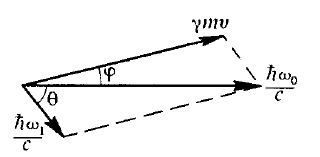
\includegraphics[width=1\linewidth]{fig1.PNG}
\caption{Схема опыта Франка и Герца} %% подпись к рисунку
\label{ris:experimoriginal} %% метка рисунка для ссылки на него
\end{minipage}
\hfill 
\begin{minipage}[h]{0.45\linewidth}
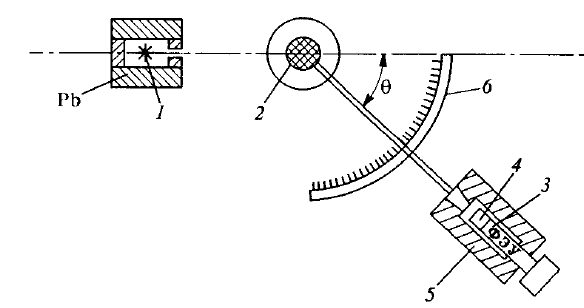
\includegraphics[width=1\linewidth]{fig2.PNG}
\caption{Схематический вид зависимости тока коллектора от напряжения на аноде}
\label{ris:experimcoded}
\end{minipage}
\end{center}
\end{figure}

\noindent При увеличении потенциала анода ток в лампе сначала растёт (зависимость, подобная ВАХ вакуумного диода). Когда энергия электронов становится достаточной для возбуждения атомов, ток коллектора резко уменьшается. Это происходит потому, что при неупругих соударениях с атомами электроны теряют свою энергию и не могут преодолеть задерживающее напряжение (около 1 В) между анодом и коллектором. При дальнейшем увеличении потенциала ток коллектора вновь возрастает: электроны, испытавшие неупругие соударения, при дальнейшем движении к аноду успевают набрать энергию, достаточную для преодоления задерживающего потенциала. Следующее замедление роста тока происходит в момент, когда часть электронов неупруго сталкивается с атомами два раза. Таким образом, на кривой зависимости тока коллектора от напряжения анода имеется ряд максимумов и минимумов, отстоящих друг от друга на равные расстояния, равные энергии первого возбуждённого состояния.

\section{Экспериментальная установка}

\begin{figure}[h]
    \centering
    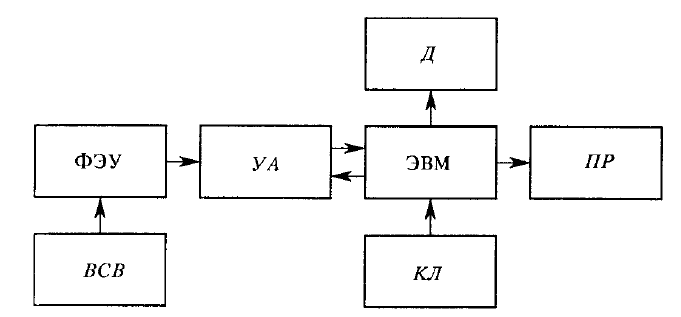
\includegraphics[width=12cm]{fig3.PNG}
    \caption{Схема экспериментальной установки}
    \label{fig:vac}
\end{figure}

На рис.3 обозначены:
\begin{itemize}
    \item А - амперметр
    \item Б7-4 - стабилизированный источник питания (подаёт напряжение накала)
    \item $K_1$ - тумблер для включения в цепь источника Б7-4
    \item Б5-10 - выпрямитель (подаёт на анод ускоряющее напряжение)
    \item $Pi_3$ - потенциометр, регулирующий величину ускоряющего напряжения
    \item $V_1$ - вольтметр, измеряющий величину ускоряющего напряжения
    \item 4,5 В - батарея КБСЛ - источник задерживающего потенциала
    \item $Pi_2$ - потенциометр, регулирующий величину задерживающего потенциала
    \item $V_2$ - вольтметр, измеряющий величину задерживающего потенциала
    \item $\mu A$ - микроамперметр - регистрирует ток в цепи коллектора
    \item $K_3$ - ключ, переключающий схему из статического режима в динамический
    \item Т - понижающий трансформатор - подаёт ускоряющий потенциал при динамическом режиме
    \item R - нагрузочный резистор
\end{itemize}


\section{Ход работы}
\subsection{Получение вольт-амперной характеристики $I_k = f(V_a)$ (динамический метод)}

1. Подготовим приборы к работе. Выберем динамический режим измерений.

\medskip

\noindent 2. При максимальном ускоряющем напряжении измерим на экране расстояние между максимумами и между минимумами осциллограммы. Проведем измерения для трёх значений задерживающего напряжения: 4, 6 и 8 В.

\begin{table}[h!]
\begin{tabular}{|r|r|r|l|l|}
\hline
\multicolumn{1}{|l|}{$V_{\text{з}}, \text{В}$} & \multicolumn{1}{l|}{$\Delta V_{min_1}, \text{В}$} & \multicolumn{1}{l|}{$\Delta V_{max_1}, \text{В}$} & $\Delta V_{min_2}, \text{В}$       & $\Delta V_{max_2}, \text{В}$       \\ \hline
4                                              & 17                                     & 15                                     &                         &                         \\ \hline
6                                              & 17                                     & 14                                     & \multicolumn{1}{r|}{14} & \multicolumn{1}{r|}{17} \\ \hline
8                                              & 18                                     & 14                                     & \multicolumn{1}{r|}{13} & \multicolumn{1}{r|}{18} \\ \hline
\end{tabular}
\end{table}
 
\begin{table}[h!]
\begin{tabular}{lll}
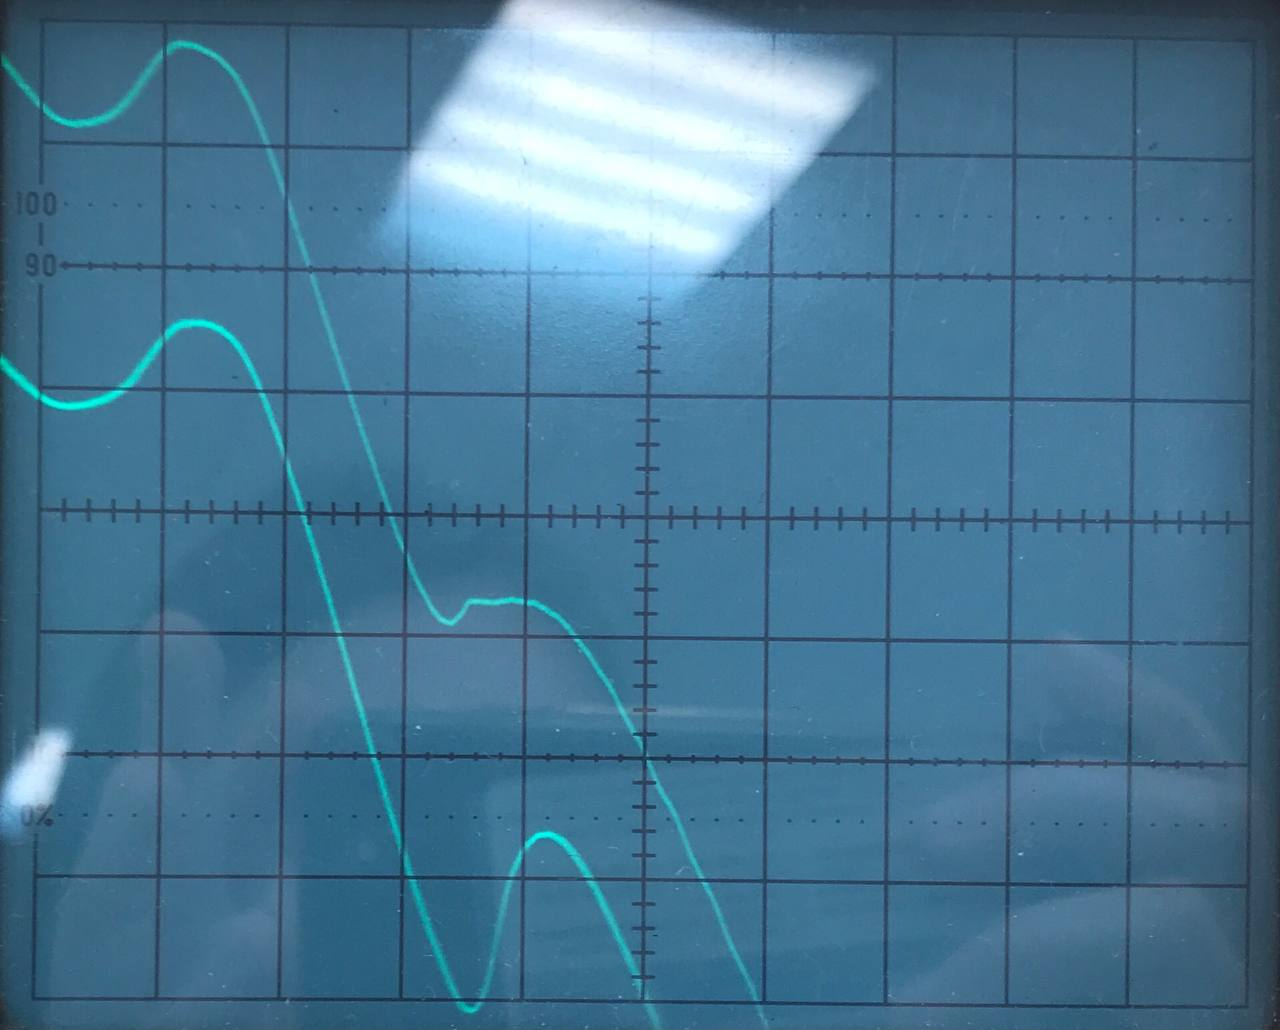
\includegraphics[width=0.3\linewidth]{1.jpg} & 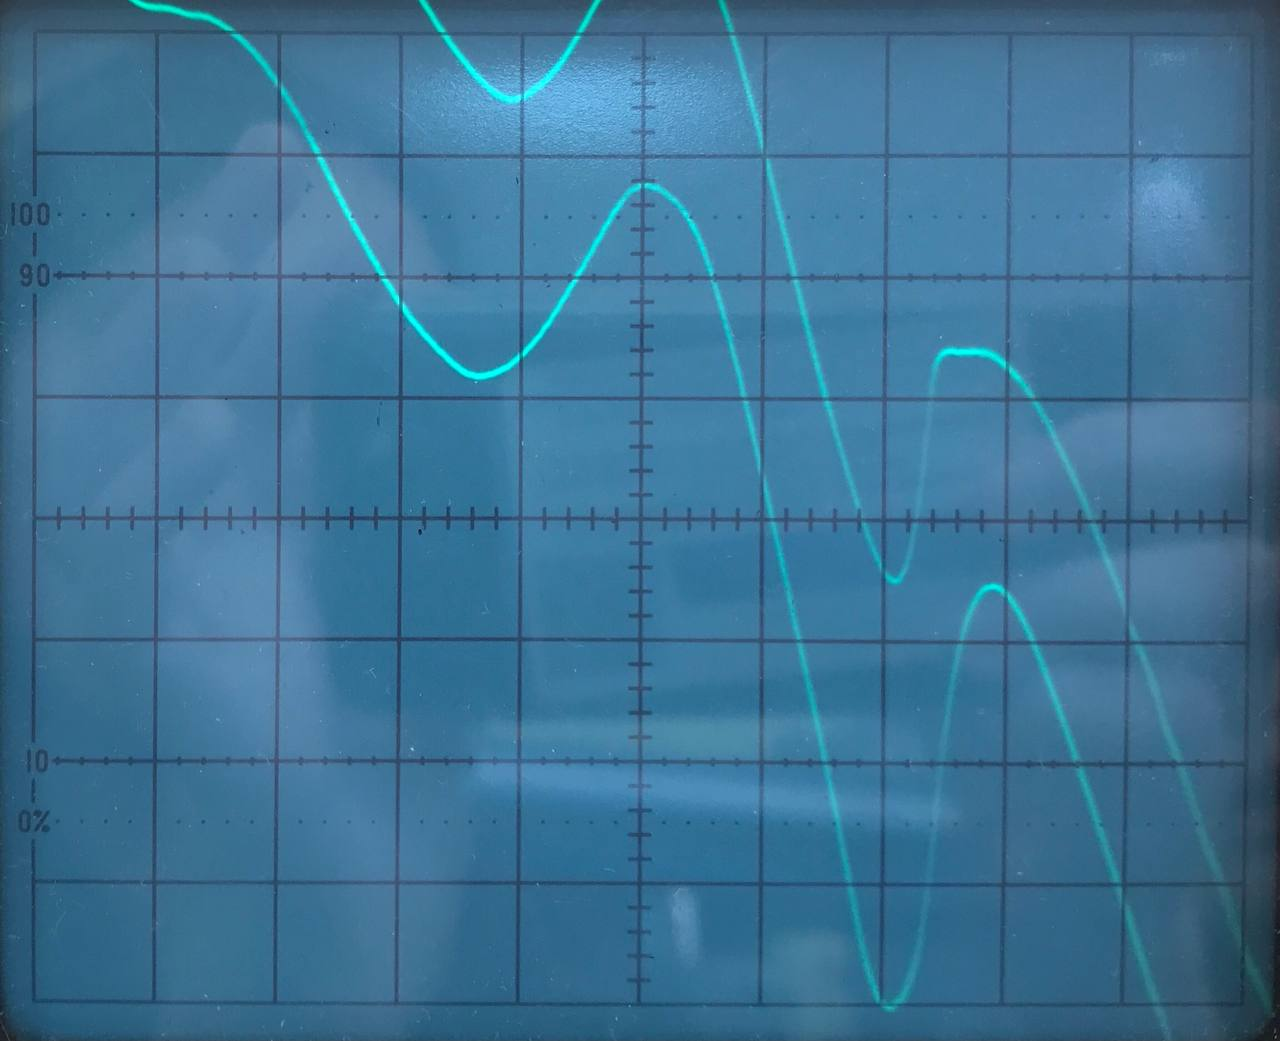
\includegraphics[width=0.3\linewidth]{2.jpg} & 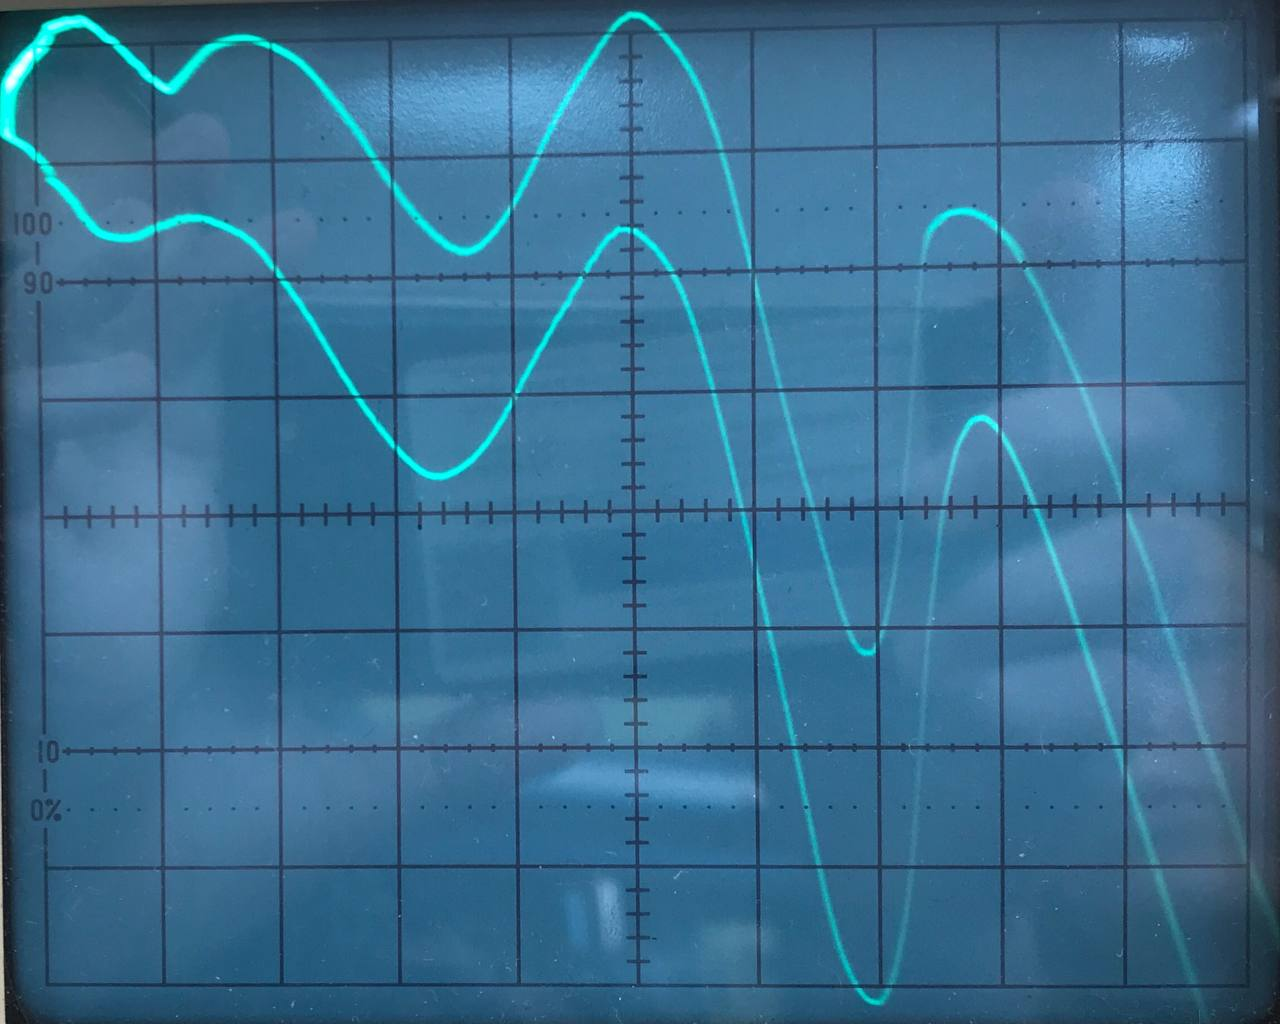
\includegraphics[width=0.3\linewidth]{3.jpg} \\
\multicolumn{1}{c}{$V_{\text{з}} = 4\text{В}$} & \multicolumn{1}{c}{$V_{\text{з}} = 6\text{В}$} & \multicolumn{1}{c}{$V_{\text{з}} = 8\text{В}$}
\end{tabular}
\end{table}

\medskip

\noindent 3. По расстоянию между минимуами и максимумами на осциллограммах определим энергию возбуждения первого уровня атома гелия в электрон-вольтах.

\noindent Оценим ошибку измерения:

    $$\sigma_
{V^2_{\text{прибора}} = \sigma_{V_{4}}^2 + \sigma_{V_{6}}^2 + \sigma_{V_{8}}^2 = 3.46 \text{ В} $$  
  $$ \sigma_{V_{\text{ср}} = \sqrt{\frac{1}{6}\sum (V_i - \overline{V})} = 1.57 \text{ В}$$


\noindent Таким образом, полученное значение:

    $$V_{\text{эксп1}} = 15.8 \pm 3.8 \text{ эВ} \text{ }(\varepsilon = 24 \%)$$ 

    $$V_{\text{табл}} = 21.6 \text{ эВ}$$ 


\subsection{Получение вольт-амперной характеристики $I_k = f(V_a)$ (статический метод)}



\noindent 1. Переключим режим на статический. 

\medskip

\noindent 2. Снимем зависимость коллекторного тока от анодного напряжения $I_k = f(V_a)$ для значений задерживающего напряжения 4, 6 и 8 В (данные см. в Приложении). 
    

\begin{figure}[h!]
    \centering
    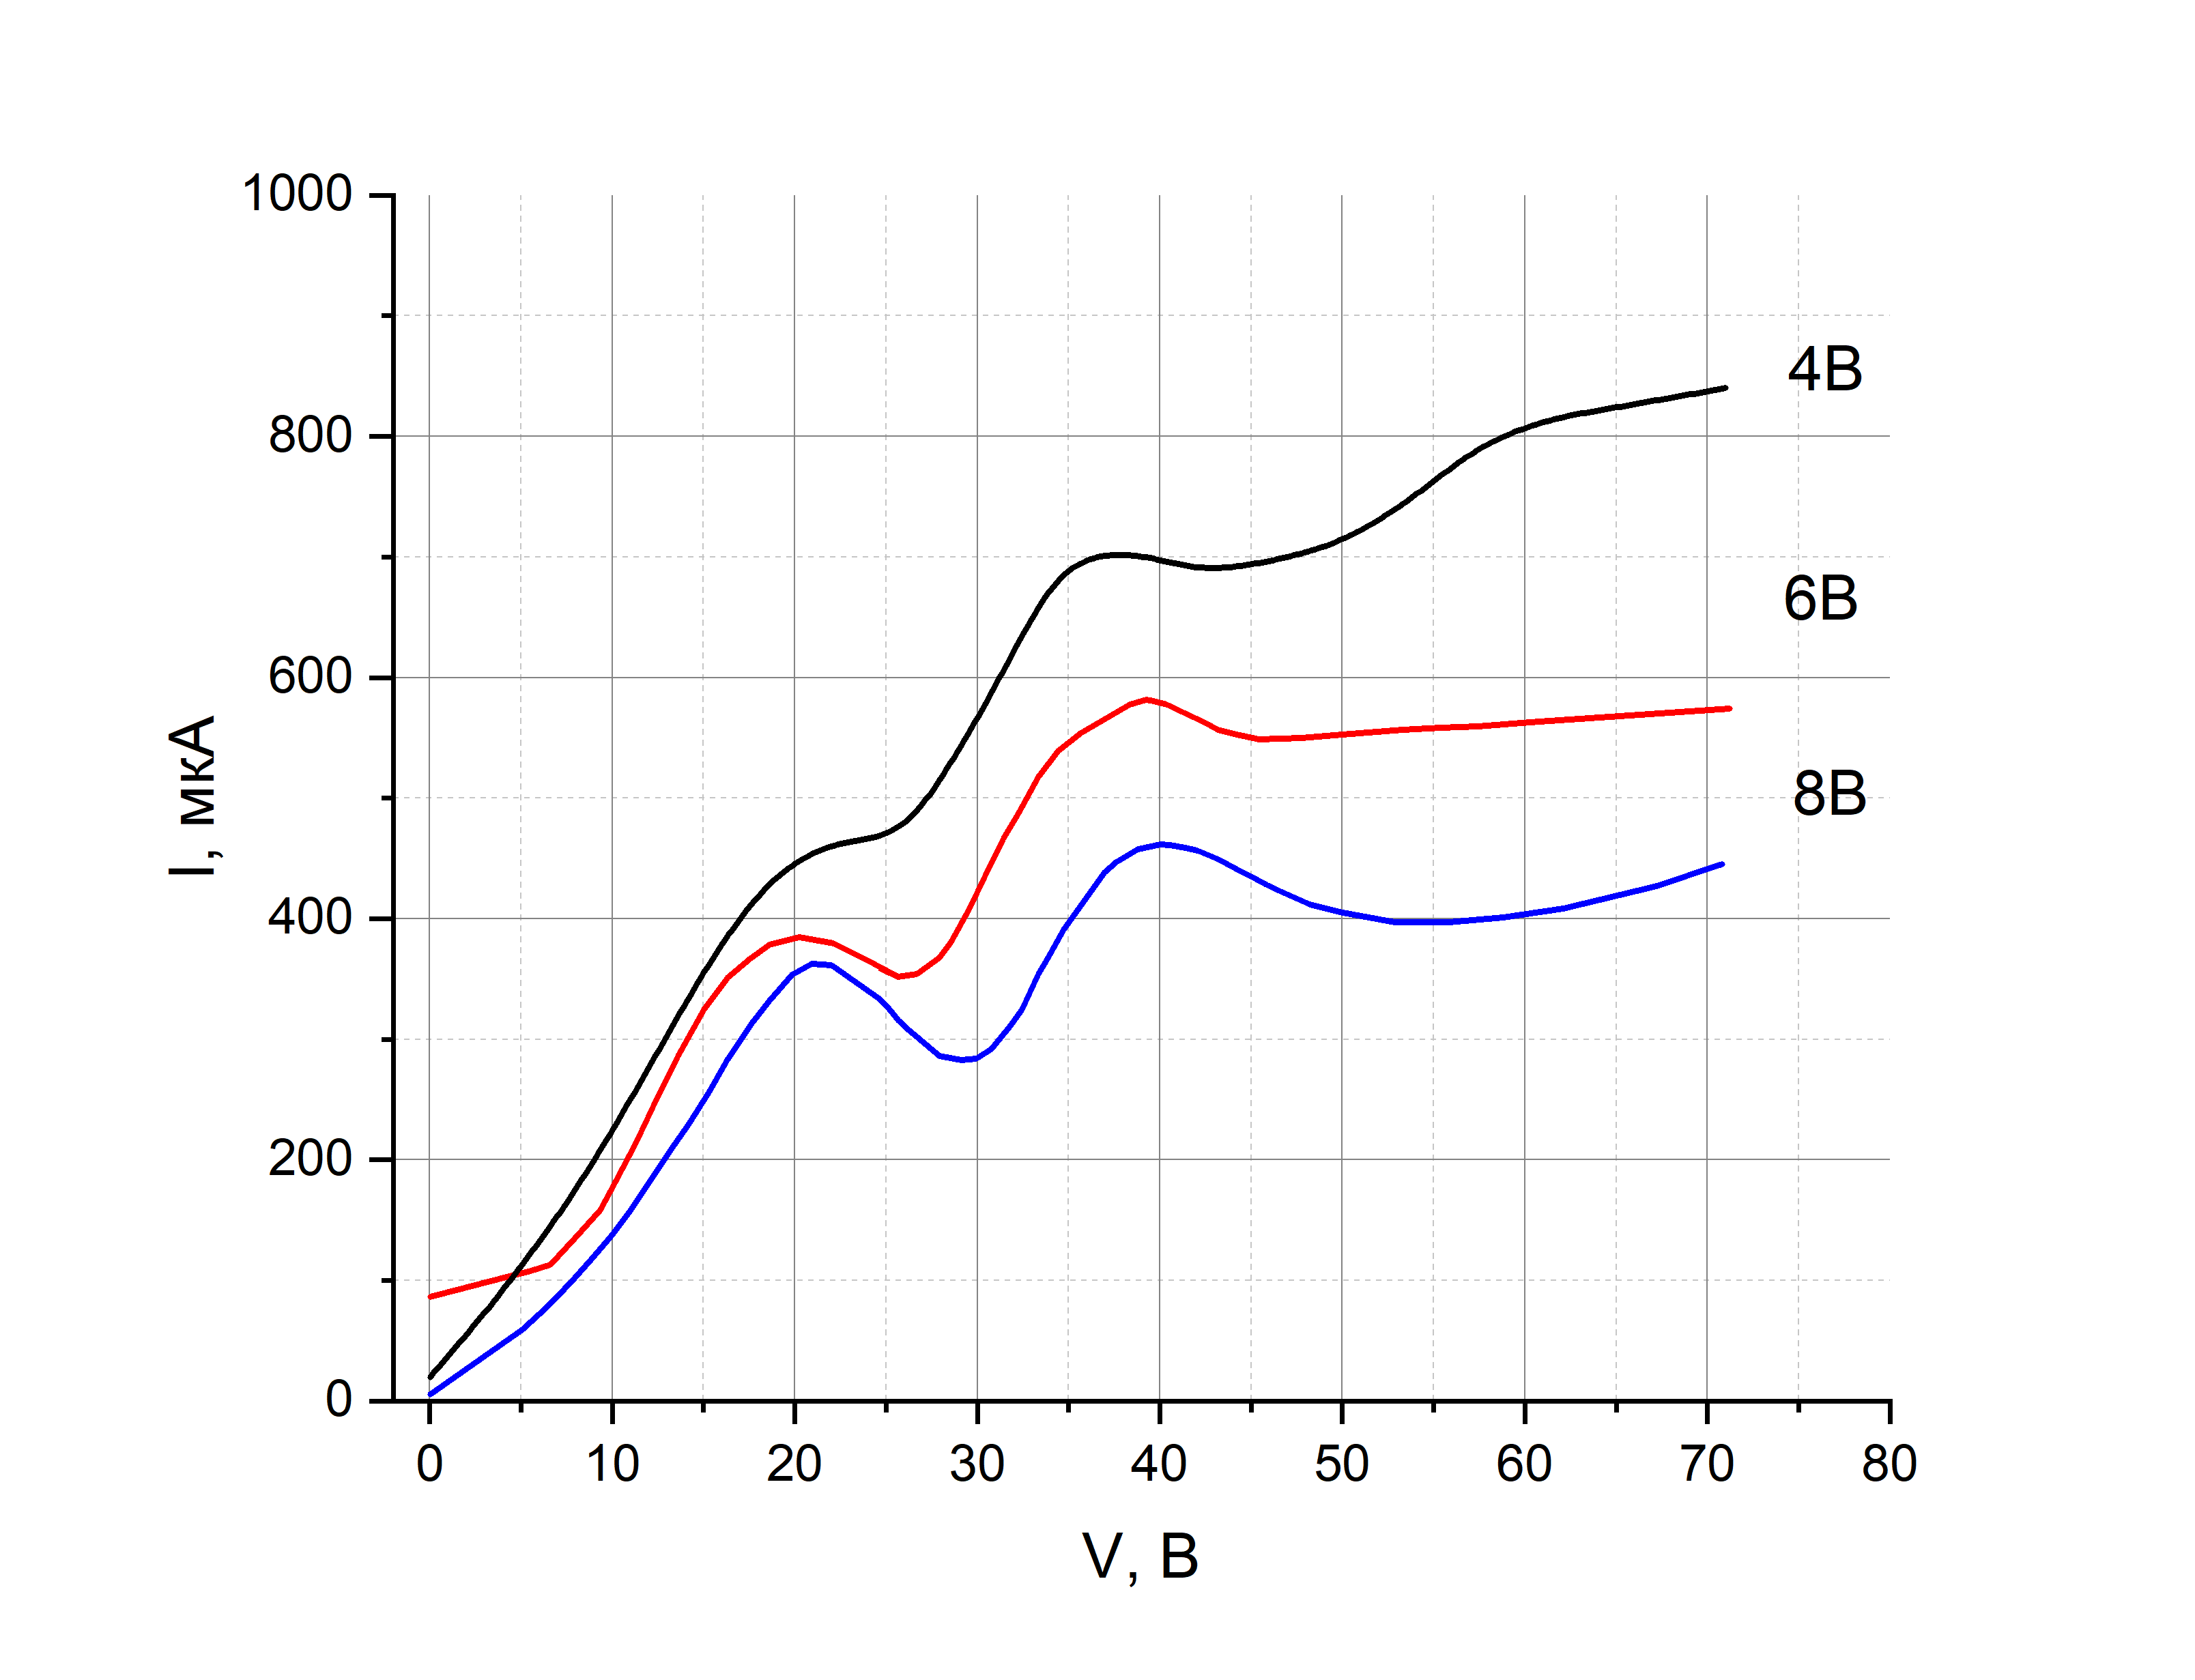
\includegraphics[scale=0.5]{I(V).png}
    \caption{Вольт-амперные характеристики при различных значениях запирающего напряжения}
    
\end{figure}

\medskip

\noindent 3. По графикам определим энергую возбуждения первого уровня атома гелия.

\medskip

\begin{table}[h!]
\begin{tabular}{|l|l|l|}
\hline
$V_\text{з}, \text{ В}$ & $\Delta V_{max}, \text{ В}$ & $\Delta V_{max}, \text{ В}$ \\ \hline
4            & 17,11            & 18,46            \\ \hline
6            & 19,01            & 19,73            \\ \hline
8            & 18,01            & 22,9             \\ \hline
\end{tabular}
\end{table}

\medskip

\noindent Оценим погрешность:

    $$\sigma_V^2_{\text{прибора}} = \sigma_V_4^2 + \sigma_V_6^2 + \sigma_V_8^2 = 3.46 \text{ В} $$  
    
\noindent Экспериментальное значение:

    $$V_{\text{эксп2}} = 19.2 \pm 3.5 \text{ эВ} \text{ }(\varepsilon = 18 \%)$$ 


\medskip

\noindent 4. Применим быстрое преобразование Фурье к вольт-амперным характеристикам на Рис. 4. Предварительно продифференцируем функции, чтобы избавиться от линейного тренда.

\medskip

\noindent Следует обратить внимание на то, что малое число периодов сигнала не позволяет точно определить фундаментальную гармонику. За погрешность примем расстояние между гармониками с наивысшей амплитудой.

\medskip

\noindent Итого получаем:

    $$V_{\text{эксп3}} = 28.1 \pm 9.2 \text{ эВ} \text{ }(\varepsilon = 33 \%)$$ 

\begin{figure}[h!]
    \centering
    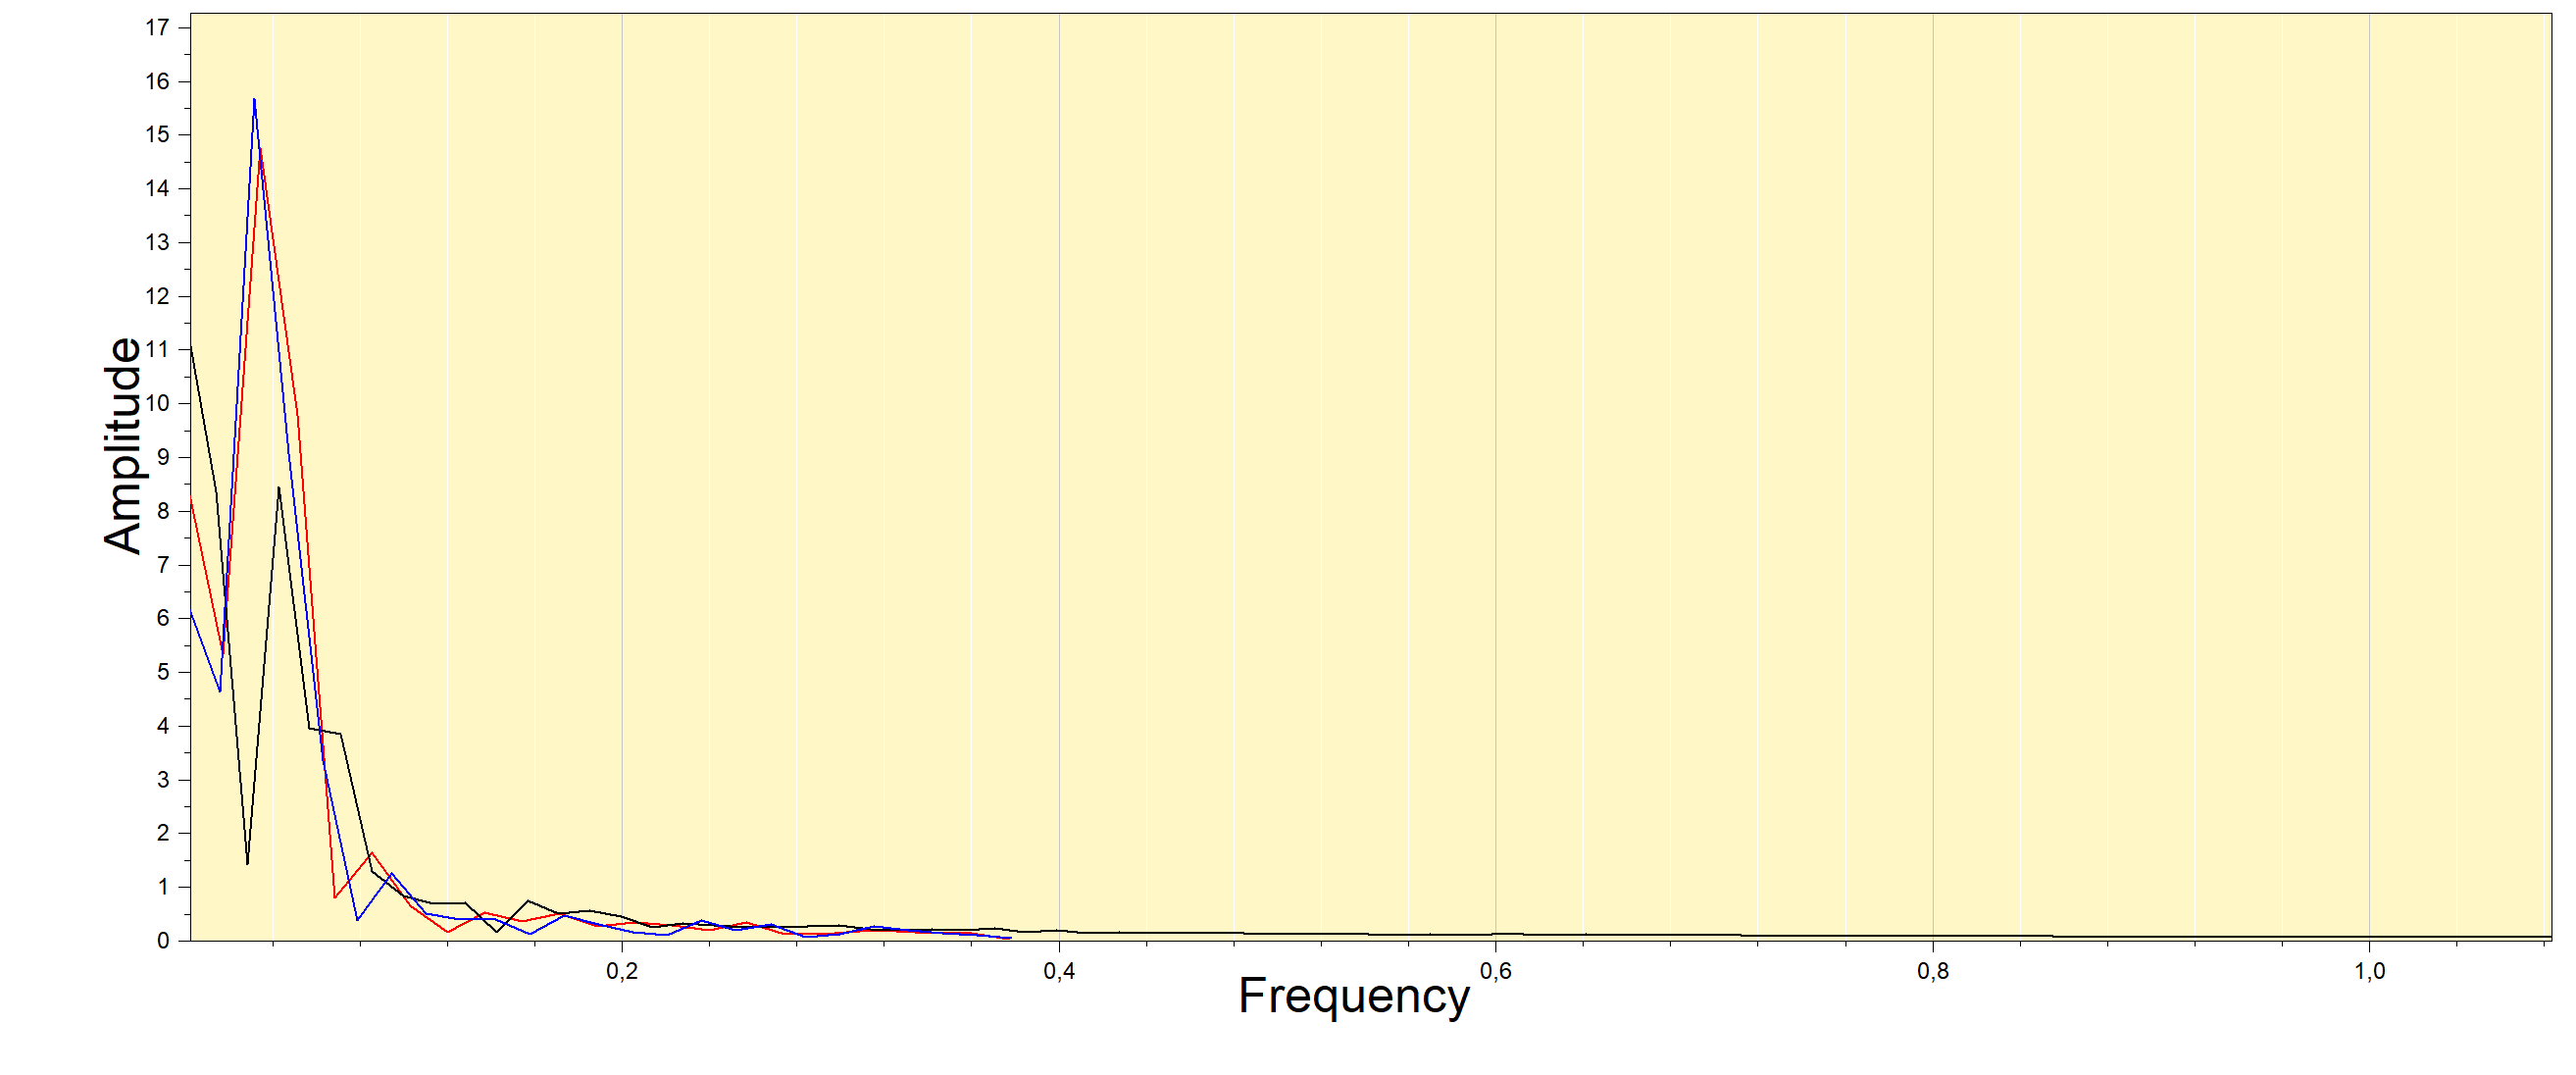
\includegraphics[scale=0.85]{FFT.png}
    \caption{FFT}
    
\end{figure}

\newpage

\section{Вывод}

\noindent В ходе работы была измерена вольт-амперная характеристика трёхэлектродной вакуумной лампы динамическим и статическим способами. По этим данным были определены потенциалы возбуждения атомов гелия. 
 
\begin{center}
    $V_\text{эксп1} = 15.8 \pm 3.8$  эВ \\
    $V_\text{эксп2} = 19.2 \pm 3.5$ эВ \\
    $V_\text{эксп3} = 28.1 \pm 9.2$ эВ \\
    $V_\text{табл} = 21.6 $ эВ
    
\end{center}

\noindent Значения совпадают с табличным по порядку величины. Статический метод показал более точные результаты -- они в пределах погрешности совпадают с табличным значением. 


\section{Приложение}
\newpage
\begin{table}[]
\begin{tabular}{|rr|rr|rr|lrrll}
\cline{1-6} \cline{8-11}
\multicolumn{2}{|c|}{4 В}                                                  & \multicolumn{2}{c|}{6 В}                                                  & \multicolumn{2}{c|}{8 В}                                                  & \multicolumn{1}{l|}{} & \multicolumn{2}{c|}{4 В}                                                  & \multicolumn{2}{c|}{8 В}                                                  \\ \cline{1-6} \cline{8-11} 
\multicolumn{1}{|l|}{$U, \text{В}$} & \multicolumn{1}{l|}{$I, \text{мкА}$} & \multicolumn{1}{l|}{$U, \text{В}$} & \multicolumn{1}{l|}{$I, \text{мкА}$} & \multicolumn{1}{l|}{$U, \text{В}$} & \multicolumn{1}{l|}{$I, \text{мкА}$} & \multicolumn{1}{l|}{} & \multicolumn{1}{l|}{$U, \text{В}$} & \multicolumn{1}{l|}{$I, \text{мкА}$} & \multicolumn{1}{l|}{$U, \text{В}$} & \multicolumn{1}{l|}{$I, \text{мкА}$} \\ \cline{1-6} \cline{8-11} 
\multicolumn{1}{|r|}{0,04}          & 26                                   & \multicolumn{1}{r|}{0,04}          & 19                                   & \multicolumn{1}{r|}{0,04}          & 19                                   & \multicolumn{1}{l|}{} & \multicolumn{1}{r|}{25,63}         & \multicolumn{1}{r|}{440}             & \multicolumn{1}{r|}{55,86}         & \multicolumn{1}{r|}{416}             \\ \cline{1-6} \cline{8-11} 
\multicolumn{1}{|r|}{1,26}          & 43                                   & \multicolumn{1}{r|}{3,75}          & 54                                   & \multicolumn{1}{r|}{5,07}          & 39                                   & \multicolumn{1}{l|}{} & \multicolumn{1}{r|}{26,46}         & \multicolumn{1}{r|}{465}             & \multicolumn{1}{r|}{58,8}          & \multicolumn{1}{r|}{438}             \\ \cline{1-6} \cline{8-11} 
\multicolumn{1}{|r|}{1,51}          & 48                                   & \multicolumn{1}{r|}{5,54}          & 87                                   & \multicolumn{1}{r|}{5,98}          & 56                                   & \multicolumn{1}{l|}{} & \multicolumn{1}{r|}{27,11}         & \multicolumn{1}{r|}{480}             & \multicolumn{1}{r|}{62,09}         & \multicolumn{1}{r|}{453}             \\ \cline{1-6} \cline{8-11} 
\multicolumn{1}{|r|}{2,03}          & 57                                   & \multicolumn{1}{r|}{6,61}          & 107                                  & \multicolumn{1}{r|}{6,83}          & 73                                   & \multicolumn{1}{l|}{} & \multicolumn{1}{r|}{27,66}         & \multicolumn{1}{r|}{497}             & \multicolumn{1}{r|}{67,21}         & \multicolumn{1}{r|}{448}             \\ \cline{1-6} \cline{8-11} 
\multicolumn{1}{|r|}{2,65}          & 67                                   & \multicolumn{1}{r|}{7,97}          & 136                                  & \multicolumn{1}{r|}{7,97}          & 95                                   & \multicolumn{1}{l|}{} & \multicolumn{1}{r|}{28,34}         & \multicolumn{1}{r|}{525}             & \multicolumn{1}{r|}{70,54}         & \multicolumn{1}{r|}{440}             \\ \cline{1-6} \cline{8-11} 
\multicolumn{1}{|r|}{2,89}          & 71                                   & \multicolumn{1}{r|}{9,35}          & 168                                  & \multicolumn{1}{r|}{8,87}          & 114                                  & \multicolumn{1}{l|}{} & \multicolumn{1}{r|}{29,24}         & \multicolumn{1}{r|}{545}             & \multicolumn{1}{r|}{70,81}         & \multicolumn{1}{r|}{438}             \\ \cline{1-6} \cline{8-11} 
\multicolumn{1}{|r|}{3,26}          & 78                                   & \multicolumn{1}{r|}{10,16}         & 187                                  & \multicolumn{1}{r|}{9,94}          & 139                                  & \multicolumn{1}{l|}{} & \multicolumn{1}{r|}{30,18}         & \multicolumn{1}{r|}{572}             &                                    &                                      \\ \cline{1-6} \cline{8-9}
\multicolumn{1}{|r|}{3,63}          & 85                                   & \multicolumn{1}{r|}{11,3}          & 217                                  & \multicolumn{1}{r|}{11}            & 164                                  & \multicolumn{1}{l|}{} & \multicolumn{1}{r|}{31,18}         & \multicolumn{1}{r|}{602}             &                                    &                                      \\ \cline{1-6} \cline{8-9}
\multicolumn{1}{|r|}{4,04}          & 92                                   & \multicolumn{1}{r|}{12,27}         & 242                                  & \multicolumn{1}{r|}{12,12}         & 193                                  & \multicolumn{1}{l|}{} & \multicolumn{1}{r|}{32,01}         & \multicolumn{1}{r|}{619}             &                                    &                                      \\ \cline{1-6} \cline{8-9}
\multicolumn{1}{|r|}{4,37}          & 98                                   & \multicolumn{1}{r|}{13,62}         & 277                                  & \multicolumn{1}{r|}{13,37}         & 227                                  & \multicolumn{1}{l|}{} & \multicolumn{1}{r|}{32,45}         & \multicolumn{1}{r|}{638}             &                                    &                                      \\ \cline{1-6} \cline{8-9}
\multicolumn{1}{|r|}{4,61}          & 103                                  & \multicolumn{1}{r|}{15,02}         & 315                                  & \multicolumn{1}{r|}{14,15}         & 245                                  & \multicolumn{1}{l|}{} & \multicolumn{1}{r|}{32,48}         & \multicolumn{1}{r|}{648}             &                                    &                                      \\ \cline{1-6} \cline{8-9}
\multicolumn{1}{|r|}{4,93}          & 110                                  & \multicolumn{1}{r|}{16,33}         & 346                                  & \multicolumn{1}{r|}{15,34}         & 277                                  & \multicolumn{1}{l|}{} & \multicolumn{1}{r|}{33,45}         & \multicolumn{1}{r|}{668}             &                                    &                                      \\ \cline{1-6} \cline{8-9}
\multicolumn{1}{|r|}{5,31}          & 117                                  & \multicolumn{1}{r|}{17,54}         & 375                                  & \multicolumn{1}{r|}{16,28}         & 304                                  & \multicolumn{1}{l|}{} & \multicolumn{1}{r|}{34,05}         & \multicolumn{1}{r|}{688}             &                                    &                                      \\ \cline{1-6} \cline{8-9}
\multicolumn{1}{|r|}{5,67}          & 124                                  & \multicolumn{1}{r|}{18,61}         & 399                                  & \multicolumn{1}{r|}{17,69}         & 335                                  & \multicolumn{1}{l|}{} & \multicolumn{1}{r|}{34,4}          & \multicolumn{1}{r|}{698}             &                                    &                                      \\ \cline{1-6} \cline{8-9}
\multicolumn{1}{|r|}{5,98}          & 130                                  & \multicolumn{1}{r|}{20,24}         & 432                                  & \multicolumn{1}{r|}{18,62}         & 359                                  & \multicolumn{1}{l|}{} & \multicolumn{1}{r|}{36,13}         & \multicolumn{1}{r|}{717}             &                                    &                                      \\ \cline{1-6} \cline{8-9}
\multicolumn{1}{|r|}{6,62}          & 143                                  & \multicolumn{1}{r|}{22,11}         & 458                                  & \multicolumn{1}{r|}{19,85}         & 384                                  & \multicolumn{1}{l|}{} & \multicolumn{1}{r|}{37,91}         & \multicolumn{1}{r|}{722}             &                                    &                                      \\ \cline{1-6} \cline{8-9}
\multicolumn{1}{|r|}{6,89}          & 150                                  & \multicolumn{1}{r|}{24,4}          & 470                                  & \multicolumn{1}{r|}{20,94}         & 405                                  & \multicolumn{1}{l|}{} & \multicolumn{1}{r|}{38,82}         & \multicolumn{1}{r|}{714}             &                                    &                                      \\ \cline{1-6} \cline{8-9}
\multicolumn{1}{|r|}{7,33}          & 159                                  & \multicolumn{1}{r|}{25,68}         & 296                                  & \multicolumn{1}{r|}{22,02}         & 424                                  & \multicolumn{1}{l|}{} & \multicolumn{1}{r|}{39,74}         & \multicolumn{1}{r|}{703}             &                                    &                                      \\ \cline{1-6} \cline{8-9}
\multicolumn{1}{|r|}{7,69}          & 167                                  & \multicolumn{1}{r|}{24,72}         & 309                                  & \multicolumn{1}{r|}{24,67}         & 437                                  & \multicolumn{1}{l|}{} & \multicolumn{1}{r|}{40,65}         & \multicolumn{1}{r|}{693}             &                                    &                                      \\ \cline{1-6} \cline{8-9}
\multicolumn{1}{|r|}{8,15}          & 177                                  & \multicolumn{1}{r|}{25,23}         & 298                                  & \multicolumn{1}{r|}{24,86}         & 444                                  & \multicolumn{1}{l|}{} & \multicolumn{1}{r|}{41,4}          & \multicolumn{1}{r|}{683}             &                                    &                                      \\ \cline{1-6} \cline{8-9}
\multicolumn{1}{|r|}{8,56}          & 187                                  & \multicolumn{1}{r|}{25,65}         & 296                                  & \multicolumn{1}{r|}{25,18}         & 230                                  & \multicolumn{1}{l|}{} & \multicolumn{1}{r|}{42,5}          & \multicolumn{1}{r|}{674}             &                                    &                                      \\ \cline{1-6} \cline{8-9}
\multicolumn{1}{|r|}{8,93}          & 196                                  & \multicolumn{1}{r|}{26,68}         & 312                                  & \multicolumn{1}{r|}{25,68}         & 210                                  & \multicolumn{1}{l|}{} & \multicolumn{1}{r|}{44,57}         & \multicolumn{1}{r|}{668}             &                                    &                                      \\ \cline{1-6} \cline{8-9}
\multicolumn{1}{|r|}{9,31}          & 206                                  & \multicolumn{1}{r|}{27,93}         & 355                                  & \multicolumn{1}{r|}{26,24}         & 202                                  & \multicolumn{1}{l|}{} & \multicolumn{1}{r|}{47,69}         & \multicolumn{1}{r|}{684}             &                                    &                                      \\ \cline{1-6} \cline{8-9}
\multicolumn{1}{|r|}{9,74}          & 216                                  & \multicolumn{1}{r|}{28,54}         & 377                                  & \multicolumn{1}{r|}{27,92}         & 213                                  & \multicolumn{1}{l|}{} & \multicolumn{1}{r|}{50,67}         & \multicolumn{1}{r|}{704}             &                                    &                                      \\ \cline{1-6} \cline{8-9}
\multicolumn{1}{|r|}{10,05}         & 225                                  & \multicolumn{1}{r|}{29,58}         & 412                                  & \multicolumn{1}{r|}{29,13}         & 245                                  & \multicolumn{1}{l|}{} & \multicolumn{1}{r|}{52,63}         & \multicolumn{1}{r|}{727}             &                                    &                                      \\ \cline{1-6} \cline{8-9}
\multicolumn{1}{|r|}{10,56}         & 238                                  & \multicolumn{1}{r|}{30,43}         & 443                                  & \multicolumn{1}{r|}{29,96}         & 277                                  & \multicolumn{1}{l|}{} & \multicolumn{1}{r|}{54,99}         & \multicolumn{1}{r|}{761}             &                                    &                                      \\ \cline{1-6} \cline{8-9}
\multicolumn{1}{|r|}{10,87}         & 246                                  & \multicolumn{1}{r|}{31,45}         & 468                                  & \multicolumn{1}{r|}{30,75}         & 308                                  & \multicolumn{1}{l|}{} & \multicolumn{1}{r|}{56,73}         & \multicolumn{1}{r|}{784}             &                                    &                                      \\ \cline{1-6} \cline{8-9}
\multicolumn{1}{|r|}{11,26}         & 256                                  & \multicolumn{1}{r|}{32,25}         & 495                                  & \multicolumn{1}{r|}{31,79}         & 343                                  & \multicolumn{1}{l|}{} & \multicolumn{1}{r|}{60,78}         & \multicolumn{1}{r|}{813}             &                                    &                                      \\ \cline{1-6} \cline{8-9}
\multicolumn{1}{|r|}{11,77}         & 269                                  & \multicolumn{1}{r|}{33,35}         & 528                                  & \multicolumn{1}{r|}{32,45}         & 371                                  & \multicolumn{1}{l|}{} & \multicolumn{1}{r|}{71}            & \multicolumn{1}{r|}{840}             &                                    &                                      \\ \cline{1-6} \cline{8-9}
\multicolumn{1}{|r|}{12,2}          & 281                                  & \multicolumn{1}{r|}{34,42}         & 562                                  & \multicolumn{1}{r|}{33,36}         & 394                                  &                       & \multicolumn{1}{l}{}               & \multicolumn{1}{l}{}                 &                                    &                                      \\ \cline{1-6}
\multicolumn{1}{|r|}{12,56}         & 290                                  & \multicolumn{1}{r|}{35,66}         & 586                                  & \multicolumn{1}{r|}{33,83}         & 413                                  &                       & \multicolumn{1}{l}{}               & \multicolumn{1}{l}{}                 &                                    &                                      \\ \cline{1-6}
\multicolumn{1}{|r|}{13,13}         & 304                                  & \multicolumn{1}{r|}{38,35}         & 603                                  & \multicolumn{1}{r|}{34,72}         & 435                                  &                       & \multicolumn{1}{l}{}               & \multicolumn{1}{l}{}                 &                                    &                                      \\ \cline{1-6}
\multicolumn{1}{|r|}{13,56}         & 316                                  & \multicolumn{1}{r|}{39,25}         & 597                                  & \multicolumn{1}{r|}{36,96}         & 458                                  &                       & \multicolumn{1}{l}{}               & \multicolumn{1}{l}{}                 &                                    &                                      \\ \cline{1-6}
\multicolumn{1}{|r|}{14}            & 328                                  & \multicolumn{1}{r|}{39,65}         & 592                                  & \multicolumn{1}{r|}{37,59}         & 476                                  &                       & \multicolumn{1}{l}{}               & \multicolumn{1}{l}{}                 &                                    &                                      \\ \cline{1-6}
\multicolumn{1}{|r|}{14,77}         & 346                                  & \multicolumn{1}{r|}{40,38}         & 583                                  & \multicolumn{1}{r|}{38,81}         & 482                                  &                       & \multicolumn{1}{l}{}               & \multicolumn{1}{l}{}                 &                                    &                                      \\ \cline{1-6}
\multicolumn{1}{|r|}{15,49}         & 364                                  & \multicolumn{1}{r|}{41,25}         & 571                                  & \multicolumn{1}{r|}{40,03}         & 473                                  &                       & \multicolumn{1}{l}{}               & \multicolumn{1}{l}{}                 &                                    &                                      \\ \cline{1-6}
\multicolumn{1}{|r|}{16,08}         & 378                                  & \multicolumn{1}{r|}{42,52}         & 555                                  & \multicolumn{1}{r|}{40,57}         & 467                                  &                       & \multicolumn{1}{l}{}               & \multicolumn{1}{l}{}                 &                                    &                                      \\ \cline{1-6}
\multicolumn{1}{|r|}{17}            & 399                                  & \multicolumn{1}{r|}{43,17}         & 548                                  & \multicolumn{1}{r|}{41,39}         & 459                                  &                       & \multicolumn{1}{l}{}               & \multicolumn{1}{l}{}                 &                                    &                                      \\ \cline{1-6}
\multicolumn{1}{|r|}{18,08}         & 424                                  & \multicolumn{1}{r|}{44,02}         & 537                                  & \multicolumn{1}{r|}{42,06}         & 452                                  &                       & \multicolumn{1}{l}{}               & \multicolumn{1}{l}{}                 &                                    &                                      \\ \cline{1-6}
\multicolumn{1}{|r|}{19,33}         & 449                                  & \multicolumn{1}{r|}{45,41}         & 526                                  & \multicolumn{1}{r|}{43,21}         & 441                                  &                       & \multicolumn{1}{l}{}               & \multicolumn{1}{l}{}                 &                                    &                                      \\ \cline{1-6}
\multicolumn{1}{|r|}{20,55}         & 469                                  & \multicolumn{1}{r|}{47,78}         & 517                                  & \multicolumn{1}{r|}{44,18}         & 424                                  &                       & \multicolumn{1}{l}{}               & \multicolumn{1}{l}{}                 &                                    &                                      \\ \cline{1-6}
\multicolumn{1}{|r|}{22,76}         & 487                                  & \multicolumn{1}{r|}{50,46}         & 531                                  & \multicolumn{1}{r|}{44,86}         & 413                                  &                       & \multicolumn{1}{l}{}               & \multicolumn{1}{l}{}                 &                                    &                                      \\ \cline{1-6}
\multicolumn{1}{|r|}{24,15}         & 411                                  & \multicolumn{1}{r|}{53,32}         & 555                                  & \multicolumn{1}{r|}{45,82}         & 401                                  &                       & \multicolumn{1}{l}{}               & \multicolumn{1}{l}{}                 &                                    &                                      \\ \cline{1-6}
\multicolumn{1}{|r|}{24,15}         & 494                                  & \multicolumn{1}{r|}{55,39}         & 577                                  & \multicolumn{1}{r|}{46,55}         & 391                                  &                       & \multicolumn{1}{l}{}               & \multicolumn{1}{l}{}                 &                                    &                                      \\ \cline{1-6}
\multicolumn{1}{|r|}{23,83}         & 492                                  & \multicolumn{1}{r|}{57,41}         & 598                                  & \multicolumn{1}{r|}{48,24}         & 380                                  &                       & \multicolumn{1}{l}{}               & \multicolumn{1}{l}{}                 &                                    &                                      \\ \cline{1-6}
\multicolumn{1}{|r|}{23,92}         & 419                                  & \multicolumn{1}{r|}{60,79}         & 622                                  & \multicolumn{1}{r|}{50,02}         & 376                                  &                       & \multicolumn{1}{l}{}               & \multicolumn{1}{l}{}                 &                                    &                                      \\ \cline{1-6}
\multicolumn{1}{|r|}{24,81}         & 423                                  & \multicolumn{1}{r|}{71,23}         & 626                                  & \multicolumn{1}{r|}{52,86}         & 390                                  &                       & \multicolumn{1}{l}{}               & \multicolumn{1}{l}{}                 &                                    &                                      \\ \cline{1-6}
\end{tabular}
\end{table}
\end{document}